\documentclass[conference]{IEEEtran}
\IEEEoverridecommandlockouts
% The preceding line is only needed to identify funding in the first footnote. If that is unneeded, please comment it out.
\usepackage{cite}
\usepackage{amsmath,amssymb,amsfonts}
\usepackage{algorithmic}
\usepackage{graphicx}
\usepackage{textcomp}
\usepackage{xcolor}
\def\BibTeX{{\rm B\kern-.05em{\sc i\kern-.025em b}\kern-.08em
    T\kern-.1667em\lower.7ex\hbox{E}\kern-.125emX}}
\graphicspath{ {./images/} }
\begin{document}

\title{Open Survey of a Convolutional Neural Network -
\\CondenseNet: An Efficient DenseNet using Learned Group Convolutions.\\
{\footnotesize Submitted as part of partial fulfillment for the Fall 2020 course: ECE 62900 - Introduction to Neural Networks. Instructor: Dr. Qingxue Zhang.}
}

\author{\IEEEauthorblockN{Priyank Kalgaonkar}
\IEEEauthorblockA{\textit{Department of Electrical and Computer Engineering} \\
\textit{Purdue School of Engineering and Technology}\\
Indianapolis, Indiana 46202, USA \\
Email: pkalgaon@purdue.edu\\
Web: www.priyankkalgaonkar.com}
}

\maketitle

\begin{abstract}
With the advent of modern embedded systems and mobile devices with limited computational power, efficient convolutional neural networks are in a great demand. A Convolutional Neural Network (CNN) is a class of Deep Neural Networks (DNN), widely used in analysis of visual images captured by an image sensor, designed to extract information and convert it in to useful representations for real-time inference of the class of the object. There are a number of different CNNs that are designed to be efficiently used on mobile devices with limited computational resources. The goal of this paper is to offer a detailed review on CondenseNet, a novel architecture developed by Gao Huang, Shichen Liu, Laurens van der Maaten, with unprecedented efficiency.\\
\end{abstract}

\begin{IEEEkeywords}
Deep Neural Network, Convolutional Neural Network, Group Convolutions.
\end{IEEEkeywords}

\section{\textbf{Introduction}}
The first working Deep Neural Network (DNN) algorithm was published by Alexey Ivakhnenko and Lapa in 1967 for supervised, deep, feed-forward,
multi-layer perceptions [1]. In 1971, Alexey Ivakhnenko published another paper describing a DNN with eight layers trained
by multi-parametric datasets [2]. Fast forwarding to the 21st century, DNN has become an important part of Computer
Vision, Natural Language Processing, Speech Recognition, Social Network Filtering, to name a few. Due to the digitization
of the human society, inexpensive cameras and Internet of Things (IoT), we now have a fairly large amount data which
enables to train a large neural network architecture to predict/infer a number of classes of objects.

Following a graph that demonstrates how scale drives the deep learning progress. The horizontal axis of the graph plots the amount of data and the vertical axis plots the performance of the learning algorithm. Thus, it can be inferred from this graph that in order to achieve a high performance of the neural network's learning algorithm, a large neural network such as AlexNet needs to be trained on a large amount of data. However, for the Traditional Learning Algorithm such as Logistic Regression, the performance at one time flats out and no longer increases. Hence, it can be trained on a small amount of data.\\

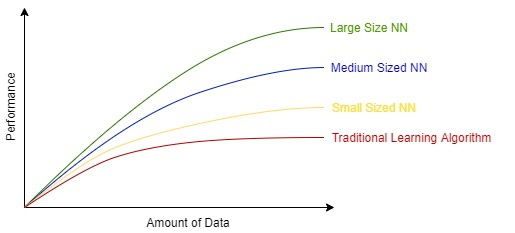
\includegraphics[scale=0.48]{graph1.jpg}\\
Figure 1: Graph that demonstrates how scale drives the deep learning process.


\section{\textbf{Evolution of Neural Networks}}

\subsection{\textbf{Logistic Regression}}
Logistic Regression is a simple form of binary classification algorithm. The input is an image and each object in the image being detected is assigned a probability between 0 and with the total sum of 1. Logistic Regression takes the input and passes it through a Sigmoid activation function that exists between 0 and 1. This Sigmoid function is responsible for classifying the input i.e. the object in the image.
\begin{center}
    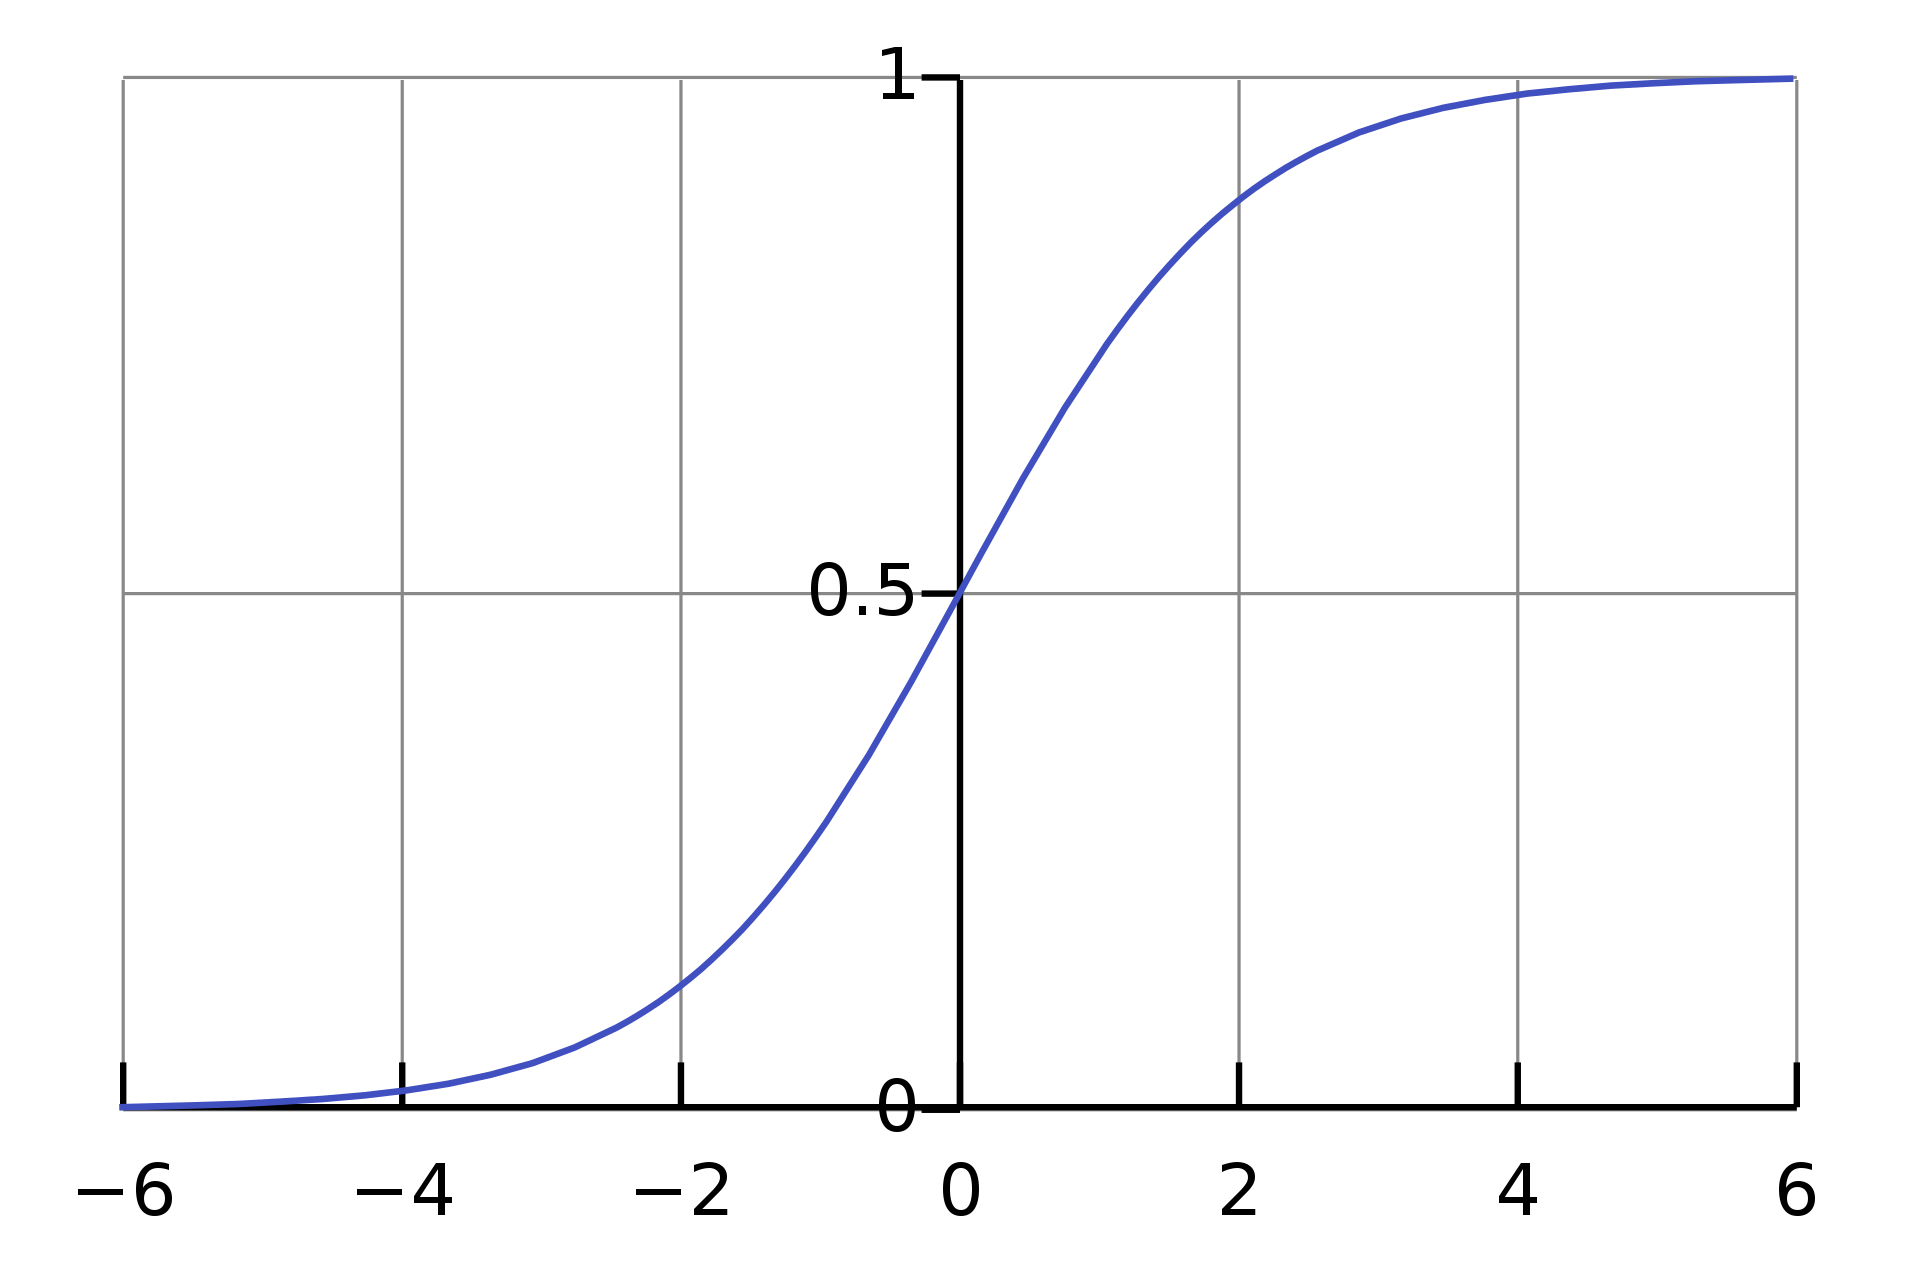
\includegraphics[scale=0.1]{1920px-Logistic-curve.svg.png}\\
\end{center}
Figure 2: Graph of Sigmoid Activation Function [3].\\

The formula for Sigmoid activation function is sig(t) =
\[\frac{1}{1+e^{-t}}\]

The Logistic Regression model takes the input as an image, for example: a 64 x 64 cat image with three channels - Red, Green & Blue, and outputs three 64 x 64 matrices. The algorithm then unrolls all these pixel values into a Feature vector $X$. The final dimension of this vector $X$ will be 64 x 64 x 3. This input is then multiplied by the Sigmoid activation function to get a value between 0 and 1 — as z increases towards positive infinity the output gets closer to 1, and as z decreases towards negative infinity the output gets closer to 0. Figure 3 below is a representation of the simple Logistic Regression Neural Network.

\begin{center}
    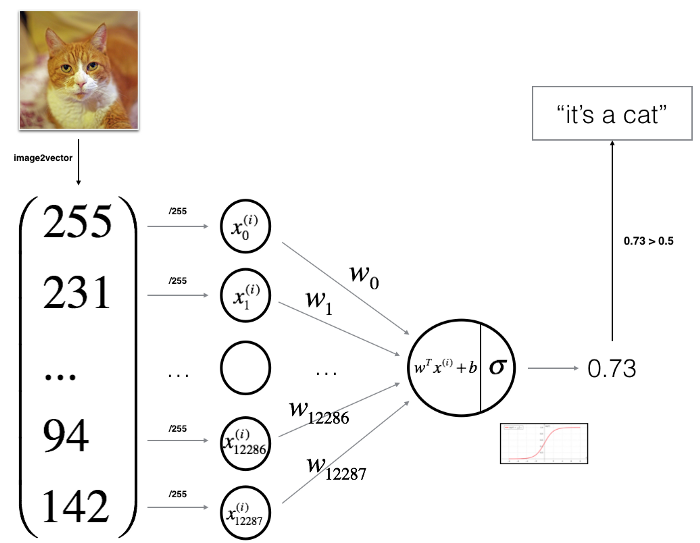
\includegraphics[scale=0.36]{LRNN.png}\\
\end{center}
Figure 3: A cat classifier that utilizes logistic regression model [7].\\

The main drawback of Logistic Regression algorithm is the assumption of linearity between the dependent and independent variables as well as the availability of structured data at all times. In the real world, the data is rarely linearly separable and always unstructured. To address these biggest pitfalls, a more complex neural networks with complicated non-linear activation functions were developed to train large amounts of data.

\subsection{\textbf{ResNet - Deep Residual Learning for Image Recognition}}
In 2015, ResNet was developed by Gao Huang, Shichen Liu, Laurens van der Maaten and Kilian Q. Weinberger to address the problem in training large (deep) neural networks. This model introduces “identity shortcut connection” that skips one or more layers, a fundamental idea behind ResNet. Instead of hoping each few stacked layers directly fit a
desired underlying mapping, the authors explicitly let these layers fit a residual mapping. Formally, denoting the desired
underlying mapping as $H(x)$, they let the stacked nonlinear layers fit another mapping of $F(x) := H(x)−x$. The original mapping is recast into $F(x)+x$. Figure 4 provides a visual representation of this novel idea.

\begin{center}
    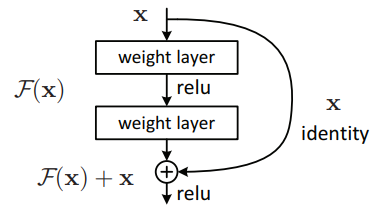
\includegraphics[scale=0.7]{ResNet.PNG}\\
\end{center}
Figure 4: Residual learning: a building block. [8]\\

The authors of ResNet argue that stacking layers should not degrade the performance of the model because identity mappings can be simply stack upon the current network and the resulting architecture would perform the same/better. Although ResNet provides a revolutionary technique that forms the basis of many popular neural network architectures today, the problem of diminishing feature reuse results in weeks of training, making it's training phase very slow and expensive.

\subsection{\textbf{(Wide)ResNet - Wide Residual Networks}}
To address the issues with ResNet, in 2016, Sergey Zagoruyko and Nikos Komodakis provided a simple yet innovative technique: multiply the number of channels at each layer by a constant. For example, WideResNet-28-10 means a ResNet has a depth of 28 layers where the number of channels is 10 times bigger at each layer. The experiments performed by the author claim to have reduced computational costs and therefore, it is more interesting to have wider ResNets than excessively deep ones.

Residual block with identity mapping can be represented by the following formula:
\[x_{l+1} = x_l +F(x_l,W_l)\]
where $x_{l+1}$ and $x_l$ are input and output of the $l$-th unit in the network, $F$ is a residual function and $W_l$ are parameters of the block. Residual network consists of sequentially stacked residual blocks. [9]

\begin{center}
    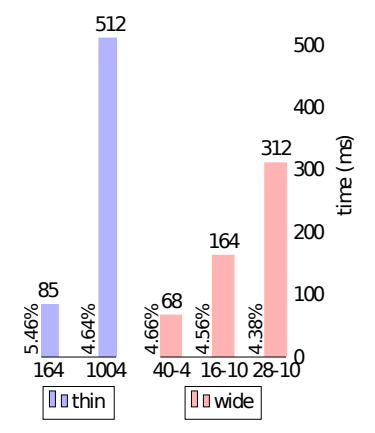
\includegraphics[scale=0.4]{WRN.PNG}\\
\end{center}
Figure 5: Time of forward+backward update per minibatch of size 32 for wide and thin networks(x-axis denotes network depth and widening factor). Numbers beside bars indicate test error on CIFAR-10, on top - time (ms). Test time is a proportional fraction of these benchmarks. Note, for instance, that wide WRN-40-4 is 8 times faster than thin ResNet1001 while having approximately the same accuracy. [9]

\subsection{\textbf{DenseNet - Densely Connected Convolutional Networks}}
In 2017, Gao Huang, Zhuang Liu, Laurens van der Maaten and Kilian Q. Weinberger took the idea of residual connections even further and published a new technique which connects each layer to every other layer in a feed-forward fashion. For each layer, the feature-maps of all preceding layers are used as inputs, and its own feature-maps are used as inputs into all subsequent layers. DenseNets have several compelling advantages: they alleviate the vanishing-gradient problem, strengthen feature propagation, encourage feature reuse, and substantially reduce the number of parameters. [10] This is a very innovative technique since it facilitates the resuse of channels and neurons (tensors) that represent information at a different level of crudeness.

DenseNets introduce three new important hyperparameters, namely [10]:
\begin{enumerate}
    \item \textbf{Growth Rate:} An important difference between DenseNet and other network architectures is that DenseNet can have very narrow layers, e.g., $k$ = 12. We refer to the hyperparameter $k$ as the growth rate of the network.
    \item \textbf{Bottleneck Layer:} A 1×1 convolution can be introduced as bottleneck layer before each 3×3 convolution to reduce the number of input feature-maps, and thus to improve computational efficiency.
    \item \textbf{Compression:} The idea of Compression is to reduce the number of channels (feature-maps) at the transition blocks. If a dense block contains $m$ feature-maps, we let the following transition layer generate $[\theta m]$ output featuremaps, where $0 <\theta \leq1$ is referred to as the compression factor. When $\theta = 1$, the number of feature-maps across transition layers remains unchanged.
\end{enumerate}

\begin{center}
    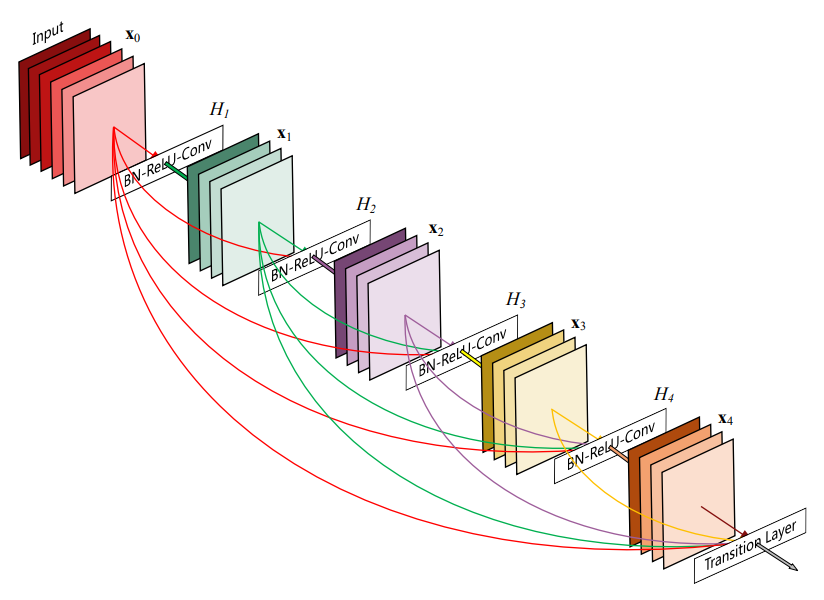
\includegraphics[scale=0.32]{DenseNEt.PNG}\\
\end{center}
Figure 6: An illustration of DenseNet. A 5-layer dense block with a growth rate of $k = 4$. Each layer takes all preceding feature-maps as input. [10]

\subsection{\textbf{CondenseNet - An Efficient DenseNet using Learned Group Convolutions}}

With the development in the area of Autonomous Vehicles, Robotics and Unmanned Ariel Vehicles such as drones, a desire for highly efficient yet accurate inferring DNN models has increased. To address this demand, in 2018, Gao Huang, Shichen Liu, Laurens van der Maaten and Kilian Q. Weinberger developed CondenseNet, an improvement over DenseNet.
The two main ideas CondenseNet uses is:
\begin{itemize}
    \item \textbf{Grouped Convolutions:} 
    \item \textbf{Connections Pruning:}
\end{itemize}













\section{\textbf{Prepare Your Paper Before Styling}}
Before you begin to format your paper, first write and save the content as a 
separate text file. Complete all content and organizational editing before 
formatting. Please note sections \ref{AA}--\ref{SCM} below for more information on 
proofreading, spelling and grammar.

Keep your text and graphic files separate until after the text has been 
formatted and styled. Do not number text heads---{\LaTeX} will do that 
for you.

\subsection{Abbreviations and Acronyms}\label{AA}
Define abbreviations and acronyms the first time they are used in the text, 
even after they have been defined in the abstract. Abbreviations such as 
IEEE, SI, MKS, CGS, ac, dc, and rms do not have to be defined. Do not use 
abbreviations in the title or heads unless they are unavoidable.

\subsection{Units}
\begin{itemize}
\item Use either SI (MKS) or CGS as primary units. (SI units are encouraged.) English units may be used as secondary units (in parentheses). An exception would be the use of English units as identifiers in trade, such as ``3.5-inch disk drive''.
\item Avoid combining SI and CGS units, such as current in amperes and magnetic field in oersteds. This often leads to confusion because equations do not balance dimensionally. If you must use mixed units, clearly state the units for each quantity that you use in an equation.
\item Do not mix complete spellings and abbreviations of units: ``Wb/m\textsuperscript{2}'' or ``webers per square meter'', not ``webers/m\textsuperscript{2}''. Spell out units when they appear in text: ``. . . a few henries'', not ``. . . a few H''.
\item Use a zero before decimal points: ``0.25'', not ``.25''. Use ``cm\textsuperscript{3}'', not ``cc''.)
\end{itemize}

\subsection{Equations}
Number equations consecutively. To make your 
equations more compact, you may use the solidus (~/~), the exp function, or 
appropriate exponents. Italicize Roman symbols for quantities and variables, 
but not Greek symbols. Use a long dash rather than a hyphen for a minus 
sign. Punctuate equations with commas or periods when they are part of a 
sentence, as in:
\begin{equation}
a+b=\gamma\label{eq}
\end{equation}

Be sure that the 
symbols in your equation have been defined before or immediately following 
the equation. Use ``\eqref{eq}'', not ``Eq.~\eqref{eq}'' or ``equation \eqref{eq}'', except at 
the beginning of a sentence: ``Equation \eqref{eq} is . . .''

\subsection{\LaTeX-Specific Advice}

Please use ``soft'' (e.g., \verb|\eqref{Eq}|) cross references instead
of ``hard'' references (e.g., \verb|(1)|). That will make it possible
to combine sections, add equations, or change the order of figures or
citations without having to go through the file line by line.

Please don't use the \verb|{eqnarray}| equation environment. Use
\verb|{align}| or \verb|{IEEEeqnarray}| instead. The \verb|{eqnarray}|
environment leaves unsightly spaces around relation symbols.

Please note that the \verb|{subequations}| environment in {\LaTeX}
will increment the main equation counter even when there are no
equation numbers displayed. If you forget that, you might write an
article in which the equation numbers skip from (17) to (20), causing
the copy editors to wonder if you've discovered a new method of
counting.

{\BibTeX} does not work by magic. It doesn't get the bibliographic
data from thin air but from .bib files. If you use {\BibTeX} to produce a
bibliography you must send the .bib files. 

{\LaTeX} can't read your mind. If you assign the same label to a
subsubsection and a table, you might find that Table I has been cross
referenced as Table IV-B3. 

{\LaTeX} does not have precognitive abilities. If you put a
\verb|\label| command before the command that updates the counter it's
supposed to be using, the label will pick up the last counter to be
cross referenced instead. In particular, a \verb|\label| command
should not go before the caption of a figure or a table.

Do not use \verb|\nonumber| inside the \verb|{array}| environment. It
will not stop equation numbers inside \verb|{array}| (there won't be
any anyway) and it might stop a wanted equation number in the
surrounding equation.

\subsection{Some Common Mistakes}\label{SCM}
\begin{itemize}
\item The word ``data'' is plural, not singular.
\item The subscript for the permeability of vacuum $\mu_{0}$, and other common scientific constants, is zero with subscript formatting, not a lowercase letter ``o''.
\item In American English, commas, semicolons, periods, question and exclamation marks are located within quotation marks only when a complete thought or name is cited, such as a title or full quotation. When quotation marks are used, instead of a bold or italic typeface, to highlight a word or phrase, punctuation should appear outside of the quotation marks. A parenthetical phrase or statement at the end of a sentence is punctuated outside of the closing parenthesis (like this). (A parenthetical sentence is punctuated within the parentheses.)
\item A graph within a graph is an ``inset'', not an ``insert''. The word alternatively is preferred to the word ``alternately'' (unless you really mean something that alternates).
\item Do not use the word ``essentially'' to mean ``approximately'' or ``effectively''.
\item In your paper title, if the words ``that uses'' can accurately replace the word ``using'', capitalize the ``u''; if not, keep using lower-cased.
\item Be aware of the different meanings of the homophones ``affect'' and ``effect'', ``complement'' and ``compliment'', ``discreet'' and ``discrete'', ``principal'' and ``principle''.
\item Do not confuse ``imply'' and ``infer''.
\item The prefix ``non'' is not a word; it should be joined to the word it modifies, usually without a hyphen.
\item There is no period after the ``et'' in the Latin abbreviation ``et al.''.
\item The abbreviation ``i.e.'' means ``that is'', and the abbreviation ``e.g.'' means ``for example''.
\end{itemize}
An excellent style manual for science writers is \cite{b7}.

\subsection{Authors and Affiliations}
\textbf{The class file is designed for, but not limited to, six authors.} A 
minimum of one author is required for all conference articles. Author names 
should be listed starting from left to right and then moving down to the 
next line. This is the author sequence that will be used in future citations 
and by indexing services. Names should not be listed in columns nor group by 
affiliation. Please keep your affiliations as succinct as possible (for 
example, do not differentiate among departments of the same organization).

\subsection{Identify the Headings}
Headings, or heads, are organizational devices that guide the reader through 
your paper. There are two types: component heads and text heads.

Component heads identify the different components of your paper and are not 
topically subordinate to each other. Examples include Acknowledgments and 
References and, for these, the correct style to use is ``Heading 5''. Use 
``figure caption'' for your Figure captions, and ``table head'' for your 
table title. Run-in heads, such as ``Abstract'', will require you to apply a 
style (in this case, italic) in addition to the style provided by the drop 
down menu to differentiate the head from the text.

Text heads organize the topics on a relational, hierarchical basis. For 
example, the paper title is the primary text head because all subsequent 
material relates and elaborates on this one topic. If there are two or more 
sub-topics, the next level head (uppercase Roman numerals) should be used 
and, conversely, if there are not at least two sub-topics, then no subheads 
should be introduced.

\subsection{Figures and Tables}
\paragraph{Positioning Figures and Tables} Place figures and tables at the top and 
bottom of columns. Avoid placing them in the middle of columns. Large 
figures and tables may span across both columns. Figure captions should be 
below the figures; table heads should appear above the tables. Insert 
figures and tables after they are cited in the text. Use the abbreviation 
``Fig.~\ref{fig}'', even at the beginning of a sentence.

\begin{table}[htbp]
\caption{Table Type Styles}
\begin{center}
\begin{tabular}{|c|c|c|c|}
\hline
\textbf{Table}&\multicolumn{3}{|c|}{\textbf{Table Column Head}} \\
\cline{2-4} 
\textbf{Head} & \textbf{\textit{Table column subhead}}& \textbf{\textit{Subhead}}& \textbf{\textit{Subhead}} \\
\hline
copy& More table copy$^{\mathrm{a}}$& &  \\
\hline
\multicolumn{4}{l}{$^{\mathrm{a}}$Sample of a Table footnote.}
\end{tabular}
\label{tab1}
\end{center}
\end{table}

\begin{figure}[htbp]
%\centerline{\includegraphics{fig1.png}}
\caption{Example of a figure caption.}
\label{fig}
\end{figure}

Figure Labels: Use 8 point Times New Roman for Figure labels. Use words 
rather than symbols or abbreviations when writing Figure axis labels to 
avoid confusing the reader. As an example, write the quantity 
``Magnetization'', or ``Magnetization, M'', not just ``M''. If including 
units in the label, present them within parentheses. Do not label axes only 
with units. In the example, write ``Magnetization (A/m)'' or ``Magnetization 
\{A[m(1)]\}'', not just ``A/m''. Do not label axes with a ratio of 
quantities and units. For example, write ``Temperature (K)'', not 
``Temperature/K''.

\section*{Acknowledgment}

The preferred spelling of the word ``acknowledgment'' in America is without 
an ``e'' after the ``g''. Avoid the stilted expression ``one of us (R. B. 
G.) thanks $\ldots$''. Instead, try ``R. B. G. thanks$\ldots$''. Put sponsor 
acknowledgments in the unnumbered footnote on the first page.

\section*{References}

Please number citations consecutively within brackets \cite{IEEEhowto:IEEEtranpage}. The 
sentence punctuation follows the bracket \cite{b2}. Refer simply to the reference 
number, as in \cite{b3}---do not use ``Ref. \cite{b3}'' or ``reference \cite{b3}'' except at 
the beginning of a sentence: ``Reference \cite{b3} was the first $\ldots$''

Number footnotes separately in superscripts. Place the actual footnote at 
the bottom of the column in which it was cited. Do not put footnotes in the 
abstract or reference list. Use letters for table footnotes.

Unless there are six authors or more give all authors' names; do not use 
``et al.''. Papers that have not been published, even if they have been 
submitted for publication, should be cited as ``unpublished'' \cite{b4}. Papers 
that have been accepted for publication should be cited as ``in press'' \cite{b5}. 
Capitalize only the first word in a paper title, except for proper nouns and 
element symbols.

For papers published in translation journals, please give the English 
citation first, followed by the original foreign-language citation \cite{b6}.

\bibliographystyle{./bibliography/IEEEtran}
\bibliography{./bibliography/IEEEabrv,./bibliography/IEEEexample}

\vspace{12pt}
\color{red}
IEEE conference templates contain guidance text for composing and formatting conference papers. Please ensure that all template text is removed from your conference paper prior to submission to the conference. Failure to remove the template text from your paper may result in your paper not being published.

\end{document}
